\documentclass[10pt,a4paper]{article}
\usepackage[utf8]{inputenc}
\usepackage{amsmath}
\usepackage{amsfonts}
\usepackage{amssymb}
\usepackage[left=2cm,right=2cm,top=2cm,bottom=2cm]{geometry}
\usepackage{graphicx}
\usepackage{wrapfig}
\usepackage{float}
\usepackage{braket}
\usepackage{mathtools}
\author{\begin{tabular}{rl}
\textbf{Course:} & PHYS 127AL \\
\textbf{Student Name:} & Nicholas Morrow \\
\textbf{Perm:} & 846646-8 \\
\textbf{Section Enrolled:} & Wien, J. - Tues. 1:00PM - 1:50PM
\end{tabular}}
\title{Project Proposal - Monophonic Analog Synthesizer}

\begin{document}
	\begin{titlepage}
		\maketitle
		\tableofcontents
	\end{titlepage}

	\section{Background}
		An analog synthesizer is a musical instrument that uses analog circuits to produce sounds through purely electronic means. Electronic sound synthesis is a fundamentally different technique from all other methods of sound generation, in the sense that other instruments typically make use of a vibrating material or resonant chamber to excite vibrational modes in the air immediately surrounding the instrument. The shape and material properties of the instrument itself act to selectively attenuate specific frequencies of the vibrational element, contributing to the instruments overall timbre. By contrast, analog synthesizers use electronic circuits as resonant elements, and the oscillatory medium is not air, but instead electric currents which circulate inside the circuit, which are then used to drive an external speaker which reproduces the synthesized waveforms acoustically. While many methods for timbre modification exist and varying widely in complexity, the timbre of a synthesizer-generated waveform is most commonly shaped by the selective addition of synthesized pure tones in a technique known as additive synthesis, or the removal of specific frequencies from harmonically rich waveforms with filtering circuits in a technique known as subtractive synthesis.
	\section{Goals and Objectives}
		The aim of the proposed project is to design, construct, and test a monophonic analog subtractive synthesizer which incorporates a voltage-controlled oscillator (VCO), voltage-controlled filter (VCF), voltage-controlled amplifier (VCA), low-frequency oscillator (LFO), envelope generators, and control inputs to allow for adjustment of several parameters related to the pitch and timbre of the sound generated by the instrument. Instead of the weekly homework assignments and laboratory exercises, a separate component of the synthesizer will be designed and simulated using SPICE in accordance with the project timeline outlined in section (4.2). A report for each module will be written, summarizing the design process and outcomes, and the individual reports will be assembled into a final report along with the outcomes of the construction and testing phase to be submitted at the end of the quarter along with the final exam.

	\section{Significance}
		The intent of this research is to learn more about the practical applications of the basic analog circuits discussed in this course, and to gain insight into the unique ways in which those basic analog circuits are applied in combination for the purpose of sound generation. It is also hoped that the basic circuit designs created during the completion of this project will provide the foundations for future revisions of this synthesizer, each of which will extend the range of achievable sounds, and allow for greater musical expression. 

	\section{Project Plan}
		In part, the construction of a synthesizer was chosen as the objective of this project because of the ease with which the final product can be separated into a list of nearly independent component circuits. Furthermore, the number of essential individual circuits required to assemble is fewer than the number of weeks in the academic quarter, which allows for the development of a schedule which allows ample time for design, simulation, testing, and assembly of the final product. 
		\newpage
		\subsection{Proposed Design}
		The proposed design attempts to find a compromise between functionality and simplicity, in the interest of the limited development time. The feature set has been chosen so as to eliminate any extraneous modulation peripherals that may convolute the development process unnecessarily, while retaining enough controllable parameters to make the instrument interesting and usable for music production.
		
		\begin{figure}[H]
			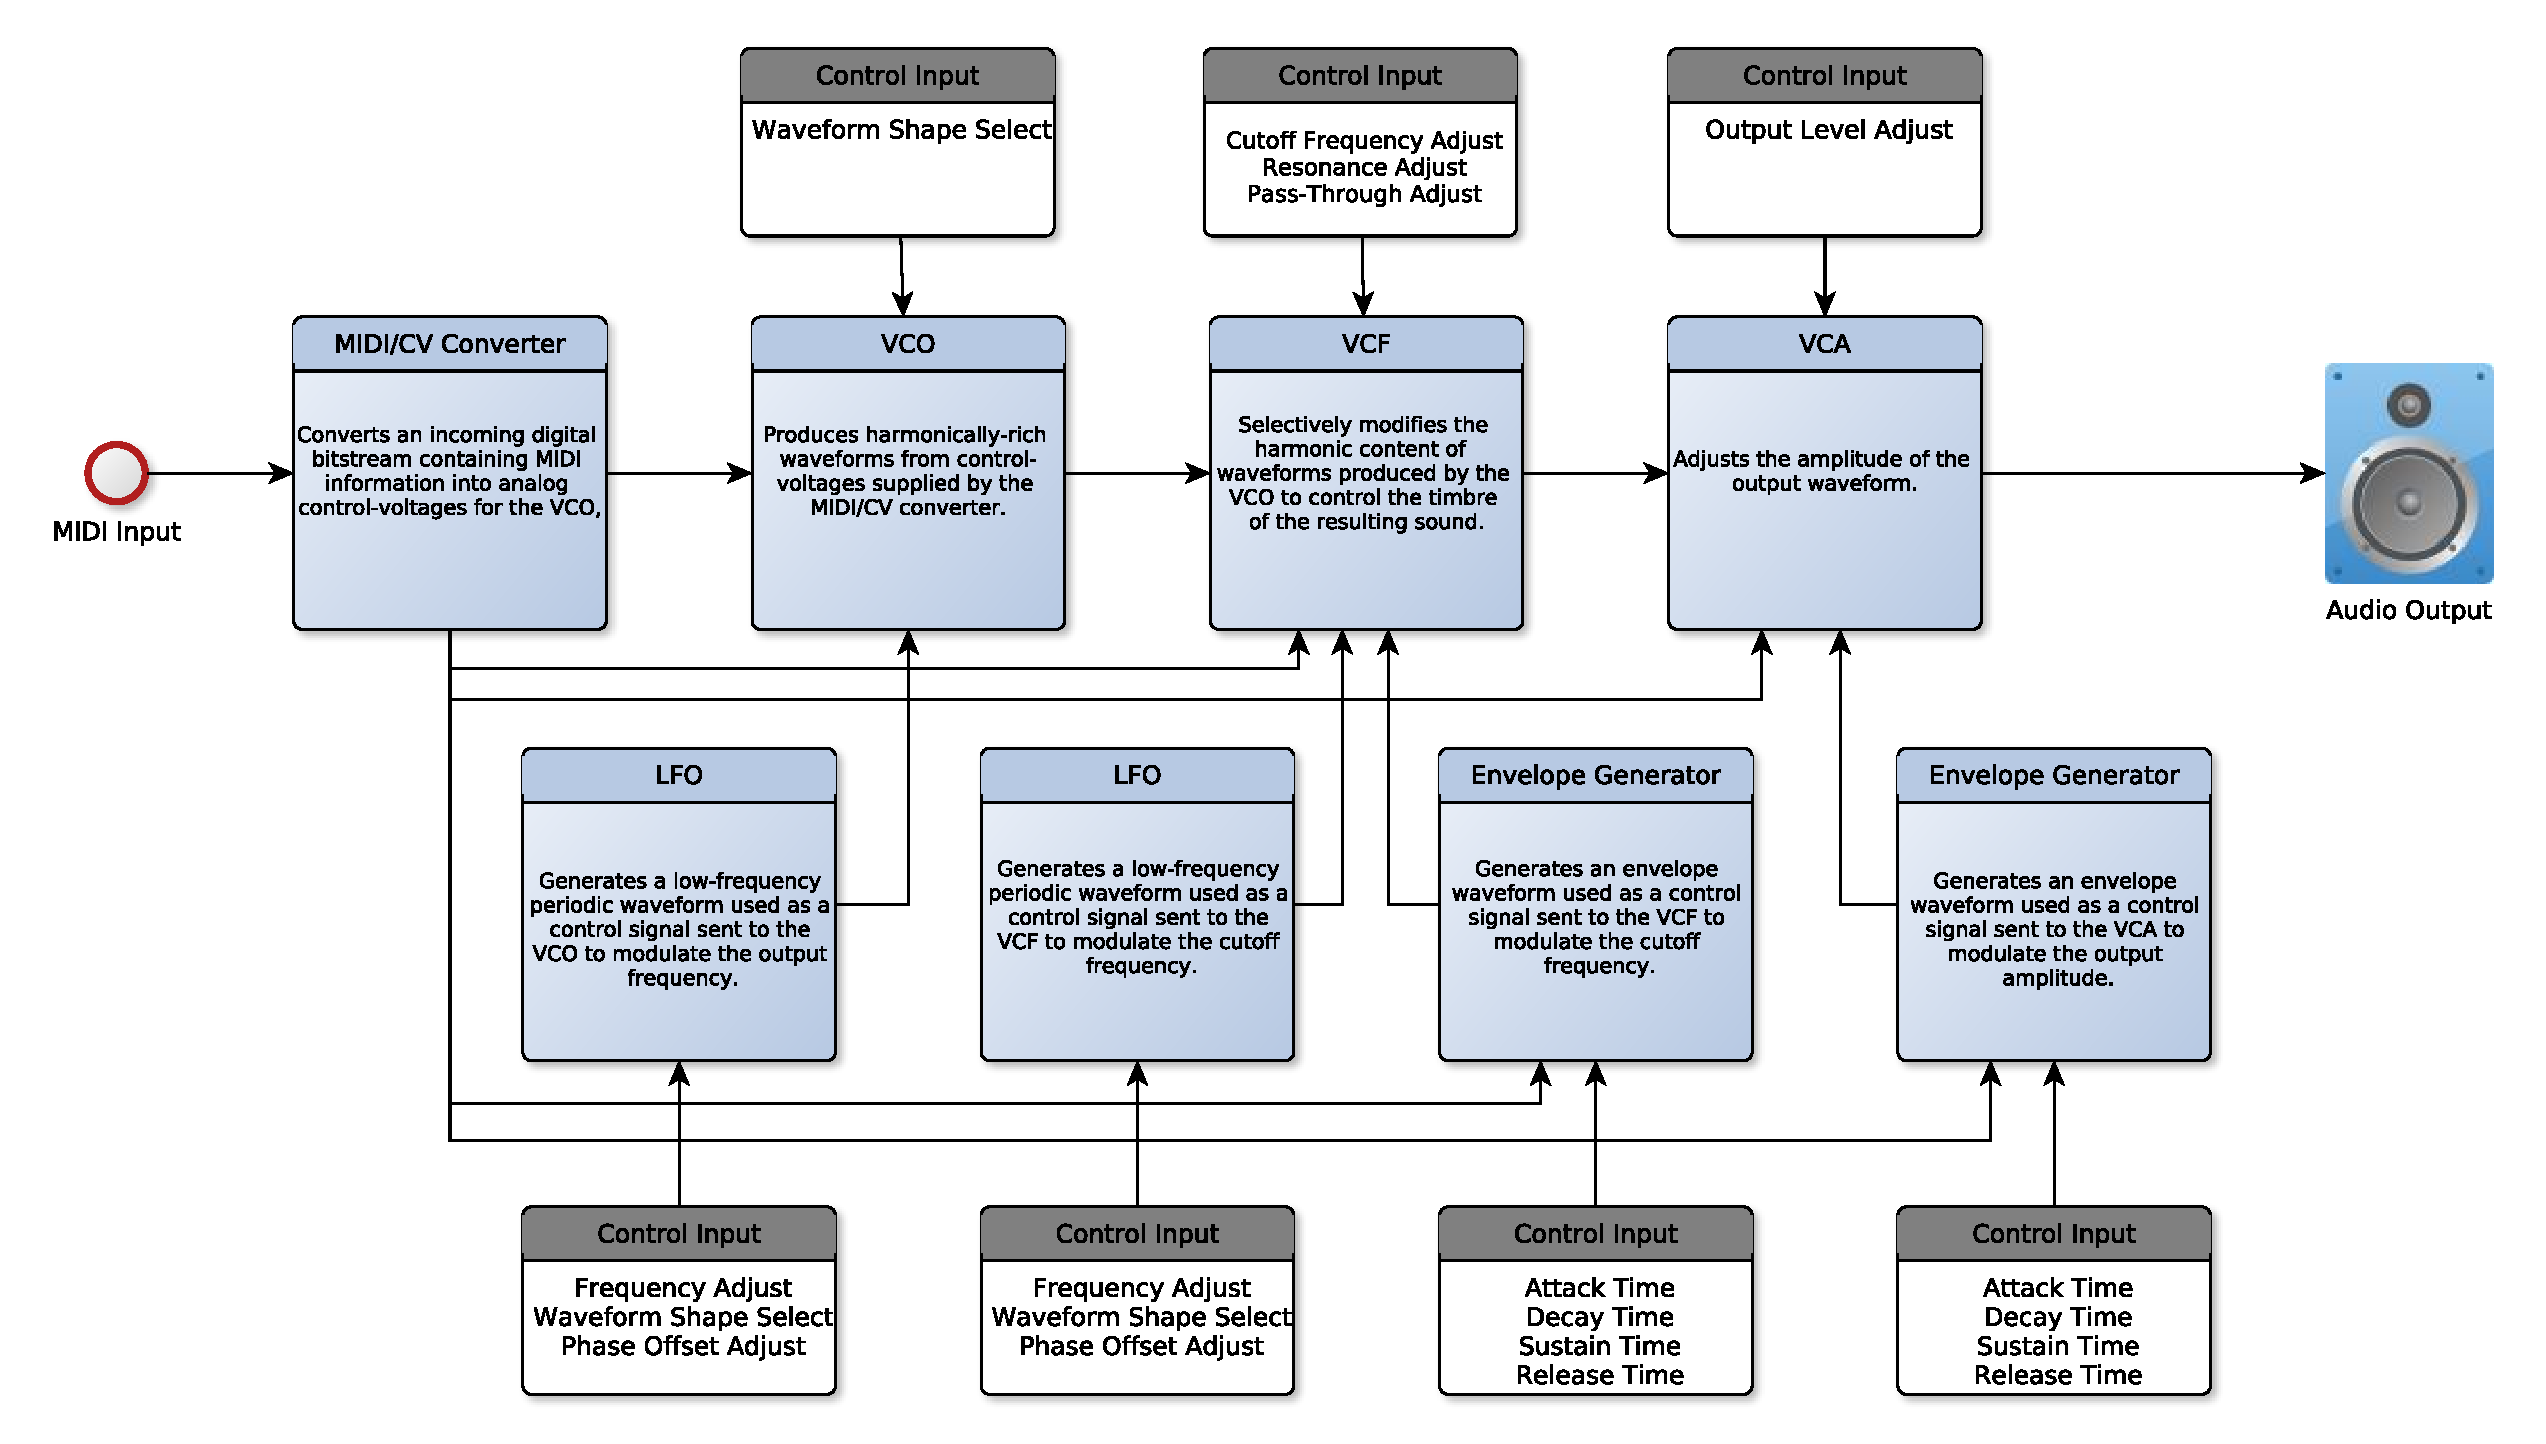
\includegraphics[width=\textwidth]{./figures/synthesizer.eps}
			\caption{Synthesizer Architecture and Signal Flow Diagram}
			\label{fig:1}
		\end{figure}
		\subsection{Timeline}
			The proposed project schedule is as follows:\\
			\begin{center}
				\begin{tabular}{|r|l|}
					\hline
					\bf{Time Period} & \bf{Task(s) To Be Performed} \\
					\hline
					Week 1 & Perform basic research and submit project proposal\\
					\hline
					Week 2 &  MIDI/CV converter design and simulation\\
					\hline
					Week 3 &  VCO design and simulation\\
					\hline
					Week 4 &  VCF design and simulation\\
					\hline
					Week 5 &  VCA design and simulation\\
					\hline
					Week 6 &  LFO design and simulation\\
					\hline
					Week 7 &  Envelope generator design and simulation\\
					\hline
					Week 8 &  Construction and Testing\\
					\hline
					Week 9 &  Construction and Testing\\
					\hline
					Week 10 &  Final exam and report submission\\
					\hline
				\end{tabular}
		\end{center}
		
\end{document}